%! Author = JustinMa
%! Date = 5/22/25

\documentclass[12pt]{article}

% Packages
\usepackage{amsmath}
\usepackage{graphicx}
\usepackage{booktabs}
\usepackage[labelfont=it, textfont=it]{caption}
\usepackage{float}
\usepackage{tikz}
\usepackage{setspace}
\usepackage{times}
\usepackage[left=1in, right=1in, top=1in, bottom=1in]{geometry}
\usepackage[colorlinks=true, linkcolor=blue, citecolor=blue, urlcolor=blue]{hyperref}

\doublespacing

% TikZ libraries and styles
\usetikzlibrary{shapes.geometric, arrows.meta, positioning, shadows}

\tikzset{
    layer/.style={
        rectangle,
        draw=black!80,
        rounded corners,
        minimum width=5cm,
        minimum height=0.6cm,
        text centered,
        text width=7cm,
        font=\small,
        drop shadow,
        fill=#1
    },
    arrow/.style={
        -{Stealth[length=2mm]},
        thick,
        shorten >=2pt,
        shorten <=2pt
    }
}

\title{Investigating Overfitting in Convolutional Neural Networks}\date{}

\begin{document}

    \maketitle

    \section*{1. Introduction}

    Neural networks are a form of machine learning models, roughly inspired by how the human brain
    processes information. They have become increasingly prevalent in our developing world, providing
    powerful and unique solutions to a wide variety of problems. However, with power also comes risk,
    as training a neural network too much on a small dataset can cause overfitting. Overfitting occurs
    when a model learns the training data too well by essentially memorizing it, causing it to perform
    well on data in its training set but poorly on test data (data that were not in the training set).
    While it might seem that simply increasing a model’s size would always boost accuracy by allowing it to
    capture more patterns, extra parameters often give the network enough capacity to store the training set
    outright when the training set is small, allowing it to overfit. Smaller networks, by contrast, are forced to find the underlying patterns
    in the data because of their limited size. In this study, we investigate whether increasing the number of
    parameters in a convolutional neural network leads to greater overfitting when trained on a small dataset, as
    measured by the difference between its accuracy on the training dataset and the test dataset.

    \section*{2. Statistical Question}

    Does increasing the number of parameters in a fixed CNN architecture cause a greater difference
    between training and testing accuracy?

    \noindent\textbf{Hypotheses:}\newline
    \centerline{$H_0: \beta = 0$} \newline
    \centerline{$H_a: \beta > 0$} \newline
    Where $\beta$ is the true slope of the population least‐squares regression line that relates number
    of parameters of the model to the difference in accuracy of the model on the train dataset and the
    test dataset (train - test).

    \section*{3. Data Collection}

    We trained 150 convolutional models, each on the same randomly selected small subset of 100 images
    from the Canadian Institute For Advanced Research - 10 dataset (CIFAR-10), which consists of 32x32 color images each labeled with one of ten classes (e.g., plane, boat, etc).
    % Each model had the same architecture, with the only difference between them being the number of parameters (\textit{see Figure 1 below}).
    The training dataset was constructed through stratified random sampling by randomly selecting 10 of each class of image, ensuring that it is representative of the entire dataset.
    The number of filters and neurons were varied between models in a way such that the sizes of the models (in parameter count) were roughly uniformly distributed, ranging from approximately 1m to 25m parameters.
    The architecture and the ratio of layer sizes were kept consistent between each model, ensuring that the only difference between them was the number of parameters (\textit{see Figure 1 below}).
    On the initialization of each model, the values of the parameters for that model were randomly set, so each model can be seen as randomly
    selected from all possible models of their respective size and architecture before training, ensuring the experiment is statistically valid.
    We controlled the parameter count by multiplying the amount of filters for the Conv2D layers and the amount of neurons
    for the hidden Dense layers by a scalar factor, $n$.

    \begin{figure}[H]
        \begin{center}
            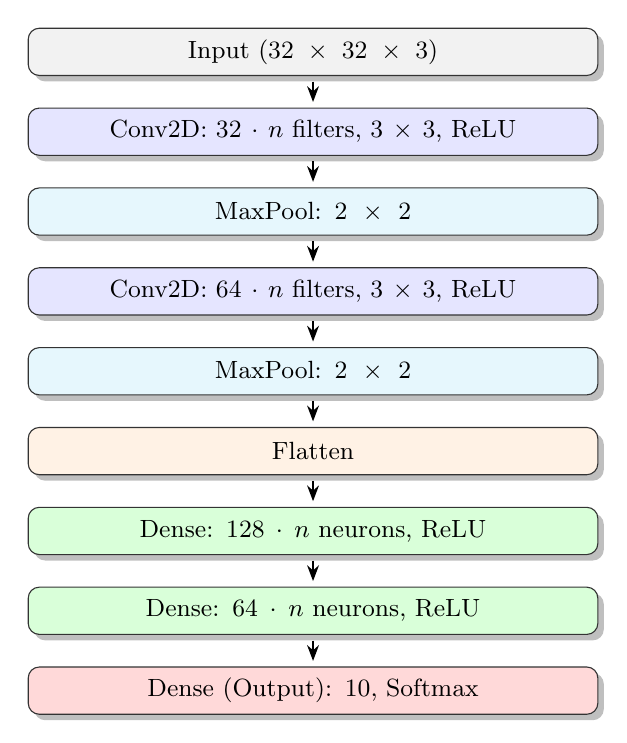
\begin{tikzpicture}[node distance=4mm and 0mm]
                \node[layer=gray!10]                     (input)  {Input $(32\times32\times3)$};
                \node[layer=blue!10,  below=of input]    (conv1)  {Conv2D: $32\cdot n$ filters, $3\times3$, ReLU};
                \node[layer=cyan!10,  below=of conv1]    (pool1)  {MaxPool: $2\times2$};
                \node[layer=blue!10,  below=of pool1]    (conv2)  {Conv2D: $64\cdot n$ filters, $3\times3$, ReLU};
                \node[layer=cyan!10,  below=of conv2]    (pool2)  {MaxPool: $2\times2$};
                \node[layer=orange!10,below=of pool2]    (flat)   {Flatten};
                \node[layer=green!15, below=of flat]    (dense1) {Dense: $128\cdot n$ neurons, ReLU};
                \node[layer=green!15, below=of dense1]  (dense2) {Dense: $64\cdot n$ neurons, ReLU};
                \node[layer=red!15,   below=of dense2]  (output) {Dense (Output): 10, Softmax};

                \draw[arrow] (input)  -- (conv1);
                \draw[arrow] (conv1)  -- (pool1);
                \draw[arrow] (pool1)  -- (conv2);
                \draw[arrow] (conv2)  -- (pool2);
                \draw[arrow] (pool2)  -- (flat);
                \draw[arrow] (flat)   -- (dense1);
                \draw[arrow] (dense1) -- (dense2);
                \draw[arrow] (dense2) -- (output);
            \end{tikzpicture}
            \caption{General Architecture of Our Models}
        \end{center}
        \label{fig:architecture}
    \end{figure}

    \noindent Each model was trained for 100 epochs on the randomly selected subset of 100 images, then evaluated
    on the full test set of the CIFAR-10 dataset, made up of 10,000 images. The difference between the train and test accuracy (train - test) was then
    computed for each model and graphed on a scatter plot with the x-axis
    as parameter count and the y-axis as the difference between train and test accuracy for each model.

    \section*{4. Data Display}
    \begin{figure}[H]
        \centering
        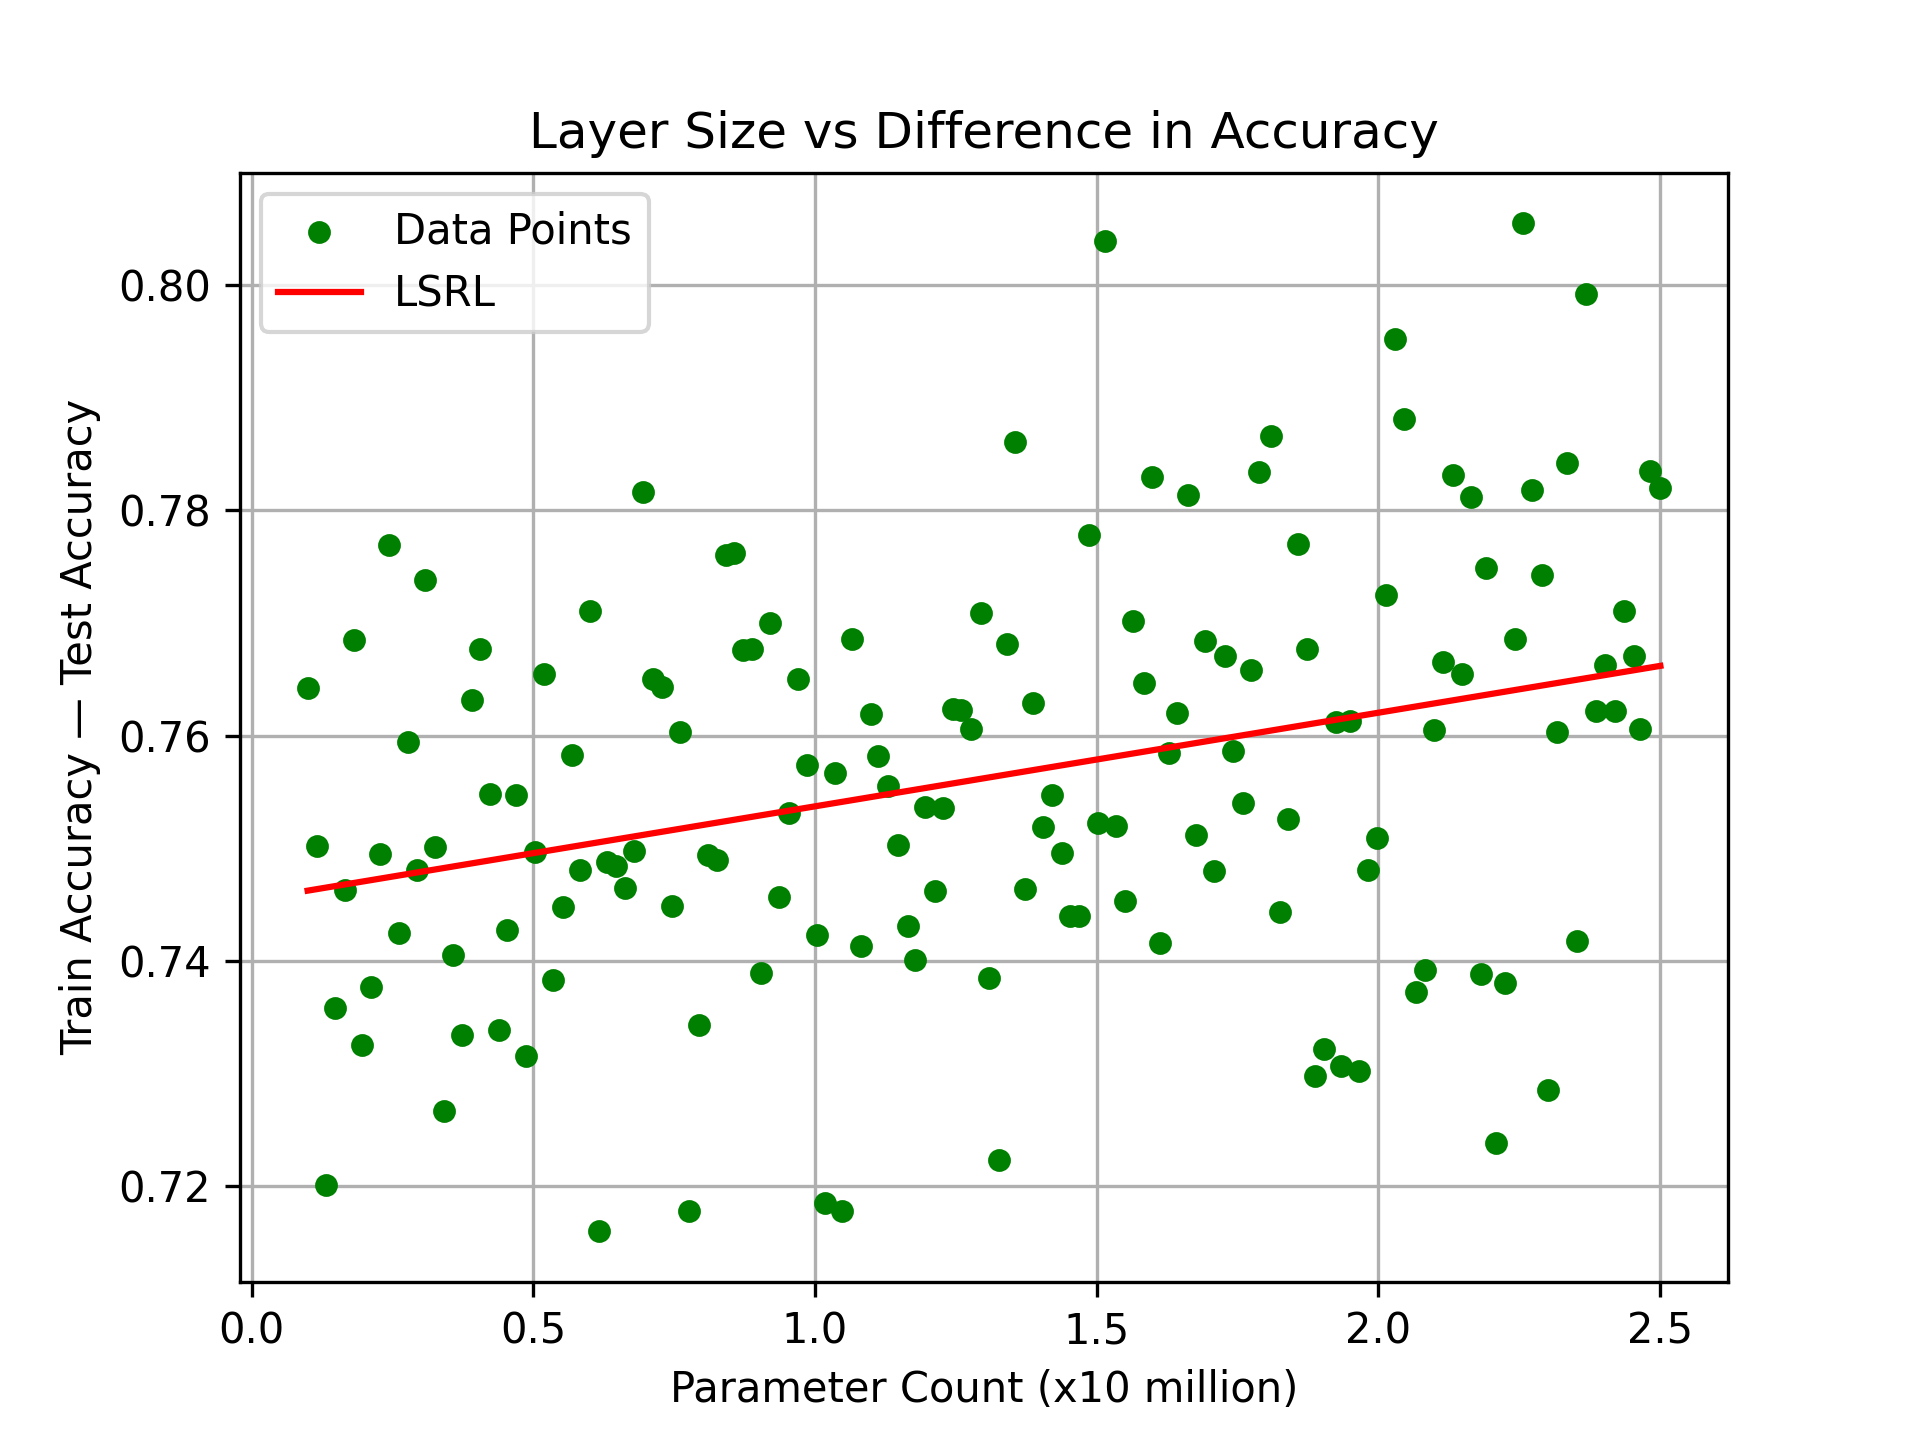
\includegraphics[width=0.7\textwidth]{Images/Scatter}
        \caption{Scatterplot of Parameter Count vs. Difference in Train and Test Accuracy (Train - Test)}
        \label{fig:scatterplot}
    \end{figure}
    There appears to be a moderate, positive, linear relationship between parameter count and difference between
    train and test accuracy (train - test). There appear to be a few possible high outliers above $x =$ 1.5 million parameters
    and a few possible low outliers above $x = 0.5$ million parameters.
    \begin{figure}[H]
        \centering
        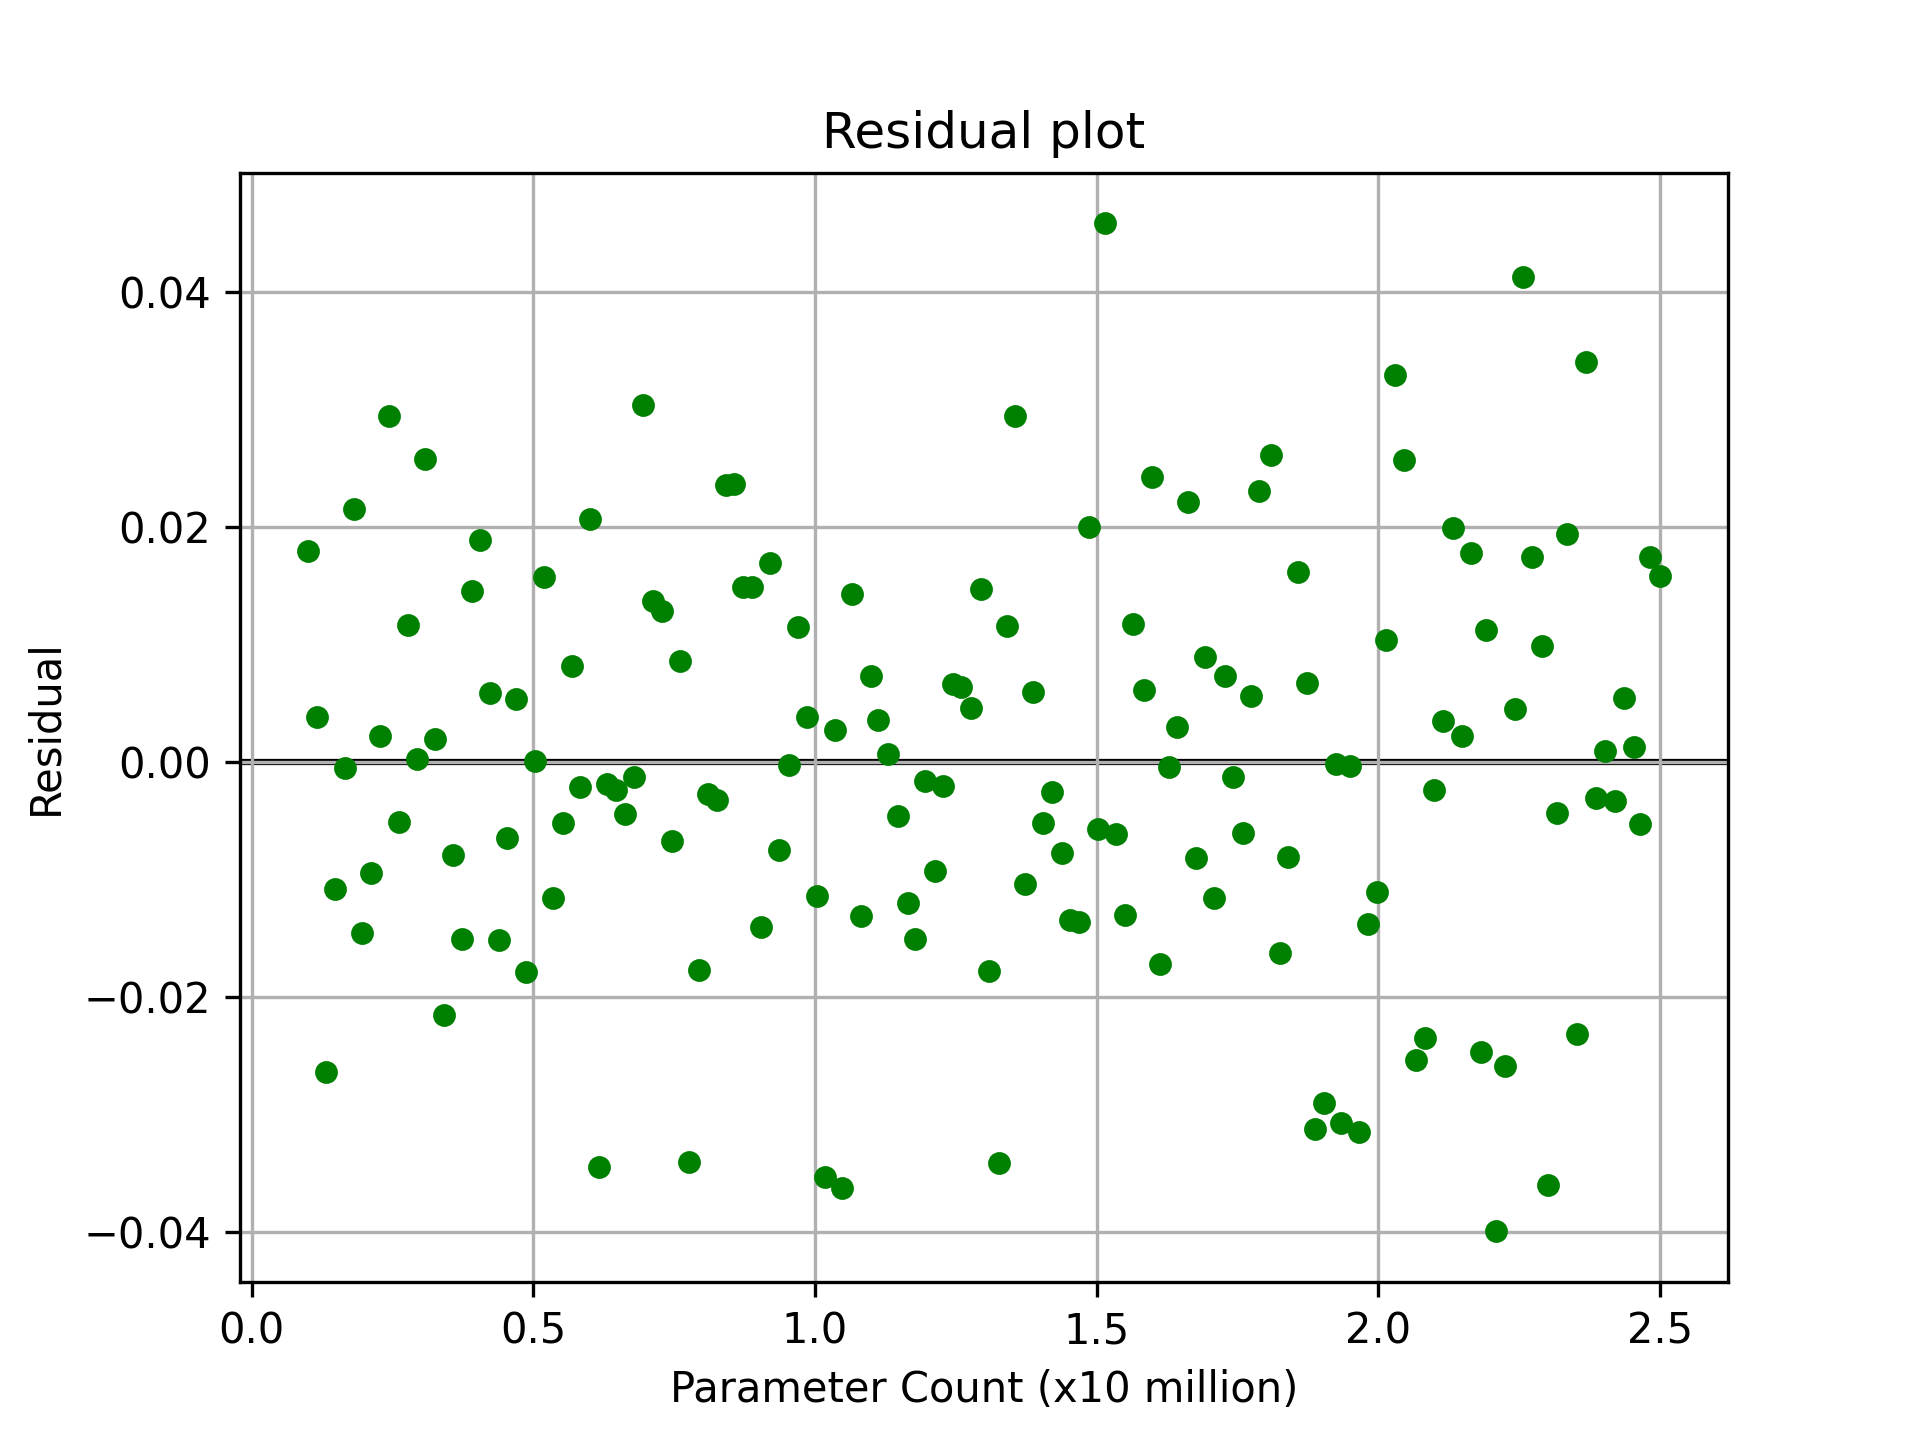
\includegraphics[width=0.7\textwidth]{Images/Resid}
        \caption{Residual Plot (Parameter Count vs. Residuals)}
        \label{fig:residuals}
    \end{figure}
    \begin{figure}[H]
        \centering
        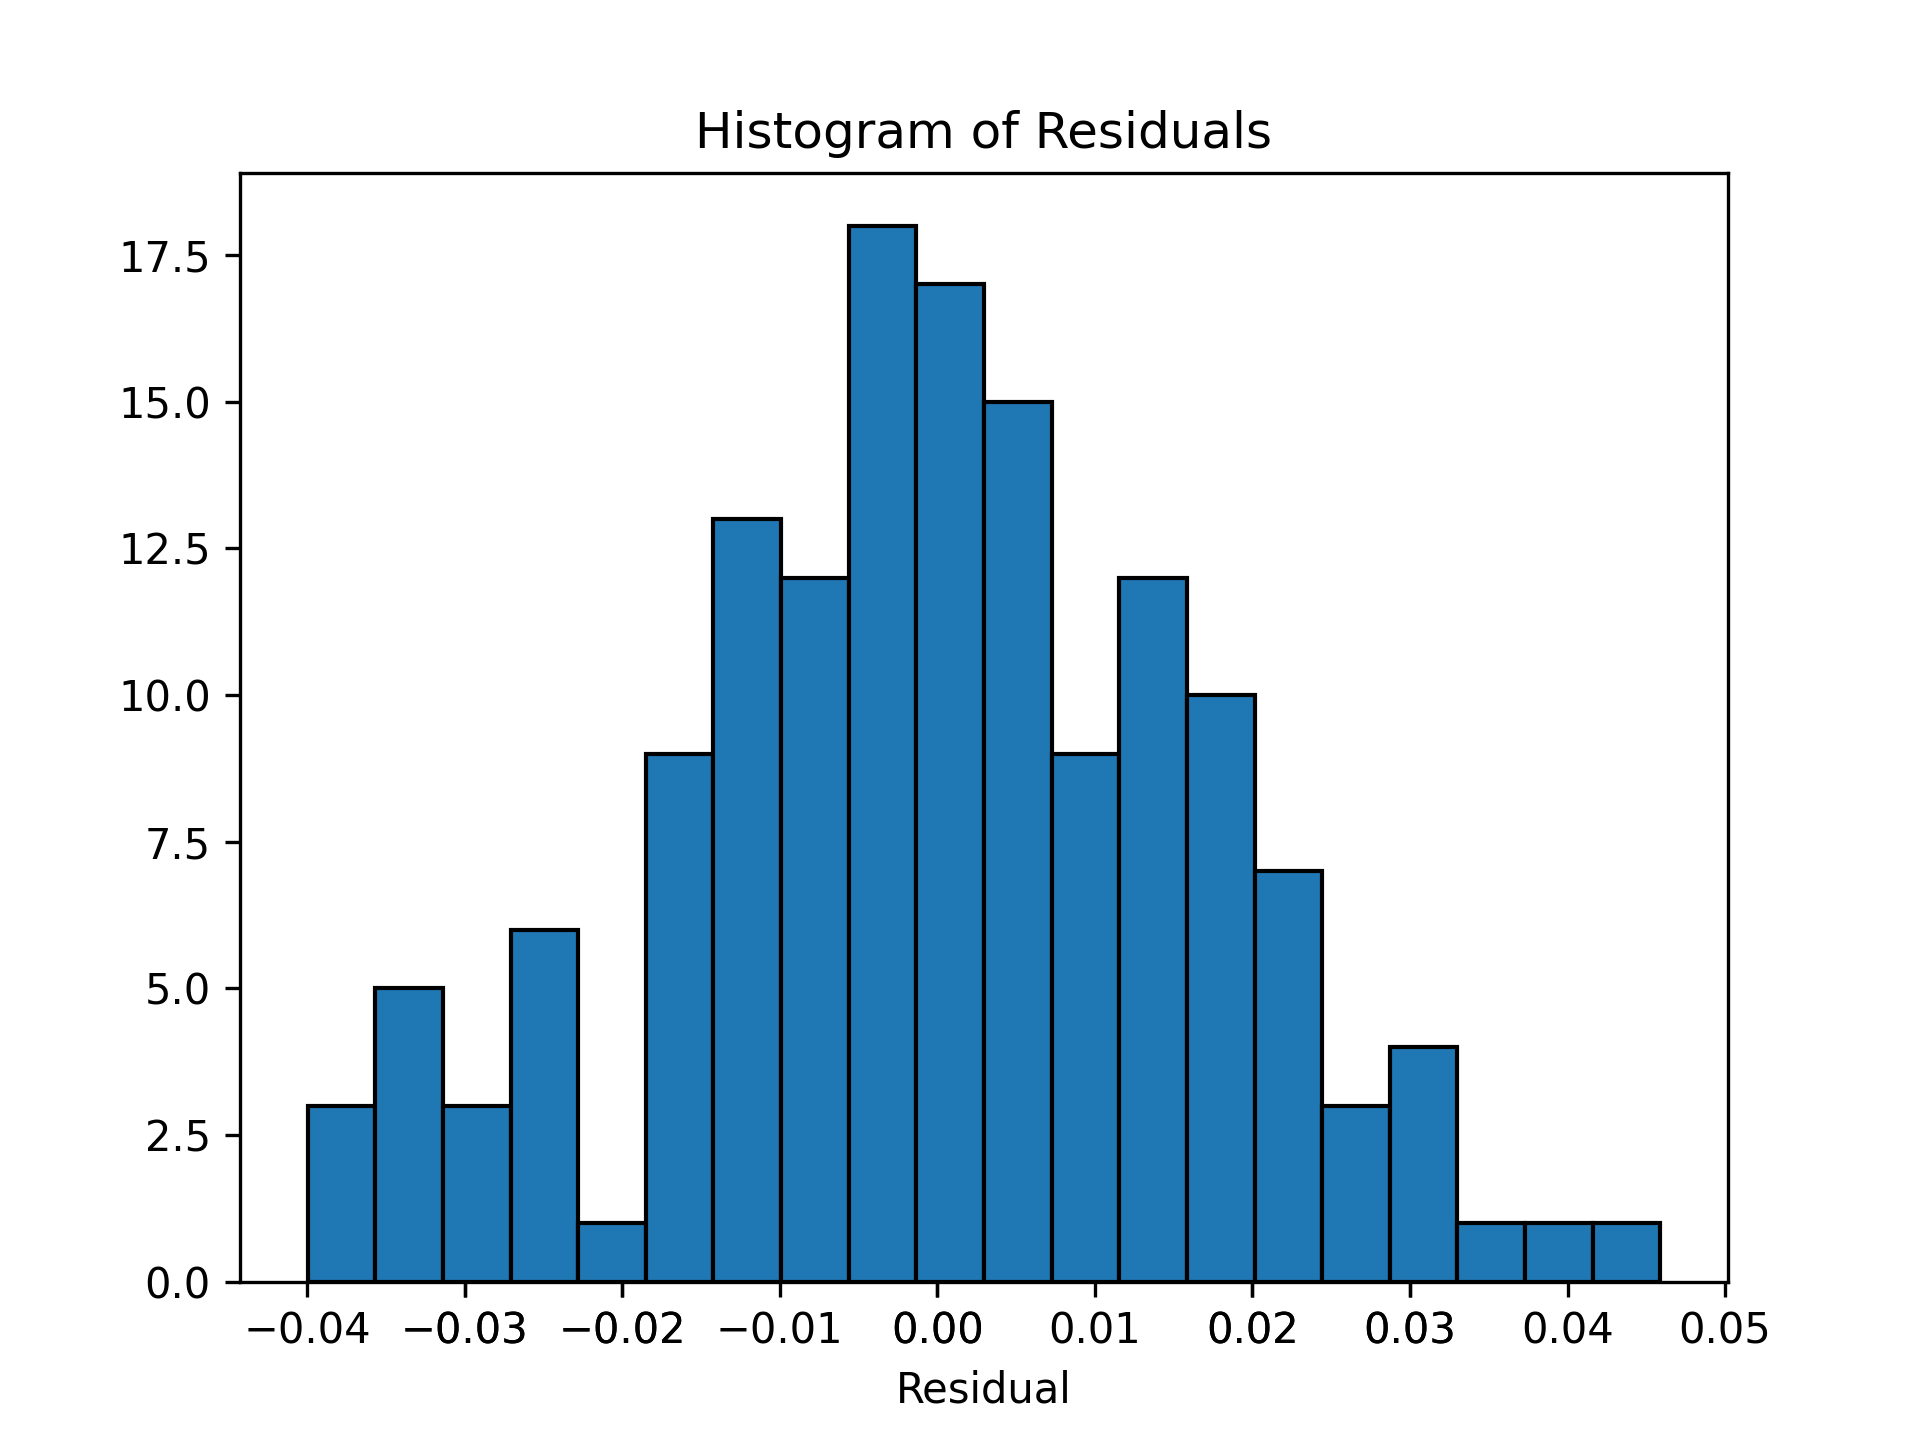
\includegraphics[width=0.7\textwidth]{Images/Resid Hist}
        \caption{Histogram of Residuals}
        \label{fig:residual_hist}
    \end{figure}
    \noindent The histogram of the residuals appears to be approximately symmetric, with a median around 0 and a range of
    $0.05-(-0.04)=0.09$. There do not appear to be any obvious outliers.

    \section*{5. Data Analysis}

    We conducted a $t$-test for the population slope $\beta$ of the least-squares regression line that relates the number of parameters in a model trained on a 100-image subset of the CIFAR-10 dataset to the difference in accuracy between training and test data (Train Accuracy $-$ Test Accuracy).

    \subsection*{5.1 Condition Check}

    \begin{quote}

    \textbf{5.1.1 Linear}

    The scatterplot of the data (\textit{\autoref{fig:scatterplot}}) shows a clear linear trend, and the residual plot (\textit{\autoref{fig:residuals}}) shows no remaining curved pattern.
    Therefore, the linearity condition is satisfied.

    \textbf{5.1.2 Independent}

    Each model was trained independently with no interaction between runs. Thus, the independence condition is met by the design of the experiment.

    \textbf{5.1.3 Normal}

    The histogram of the residuals (\textit{\autoref{fig:residual_hist}}) shows no strong skew and no obvious outliers,
    so the normality condition is met.

    \textbf{5.1.4 Equal Variance}

    The residual plot (\textit{\autoref{fig:residuals}}) shows shows no noticeable $<$ or $>$ shape, so the equal variance condition is satisfied.

    \textbf{5.1.5 Random}

    The parameters of the model were randomized on initialization, so each model can be seen as randomly selected from the population
    of models of the same size and structure.

    \end{quote}

    \subsection*{5.2 Calculations}

    \subsubsection*{5.2.1 Standard Error}

    We used the following equation to calculate the Standard Error $SE_\beta$ of the slope $\beta$:
    \[
        \mathrm{SE}_{\beta}
        =
        \frac{
            \displaystyle S
        }{
            \displaystyle S_x \sqrt{n - 1}
        }
    \]
    \noindent We need the standard deviation of the residuals and of the parameter counts to find $SE_\beta$, which we found like this:
    \begin{align*}
        \mathrm{S} &=
        \sqrt{
            \frac{
                \sum_{i=1}^n (y_i - \hat{y}_i)^2
            }{
                n - 2
            }
        } \\[1em]
        \mathrm{S}_x &=
        \sqrt{
            \frac{
                \sum_{i=1}^n (x_i - \bar{x})^2
            }{
                n - 1
            }
        }
    \end{align*}
    \noindent After plugging in all of the data from the 150 models, we got $S = 0.01703$ and $S_x = 0.6972$.
    Now we can use those to find $SE_\beta$:
    \[
        \mathrm{SE}_{\beta}
        =
        \frac{
            \displaystyle 0.01703
        }{
            \displaystyle 0.6972 \sqrt{150 - 1}
        }
        =
        0.002008
    \]

    \subsubsection*{5.2.2 $t$-statistic}
    \noindent And now we can find the t-statistic, which represents how many standard deviations away our sample slope $b$ is from the population slope $\beta$, assuming that $\beta=0$:
    \begin{gather*}
        \mathrm{t} = \frac{b}{SE_\beta} \\[1em]
        \mathrm{t} = \frac{0.008312}{0.002008} = 4.139
    \end{gather*}

    \subsubsection*{5.2.3 $p$-value}
    \noindent Now that we have the t-statistic, we can use it to find the $p$-value, which represents the probability of getting a test statistic
    of $4.139$ or higher, assuming that the population slope $\beta$ is $0$. Because we have 150 data points, we have $150 - 2 = 148$ degrees of freedom.
    Thus, we calculate the $p$-value by finding the amount of area under a $t$-distribution with 148 degrees of freedom, above $t=4.139$. The graph below demonstrates this:

    \begin{figure}[H]
        \centering
        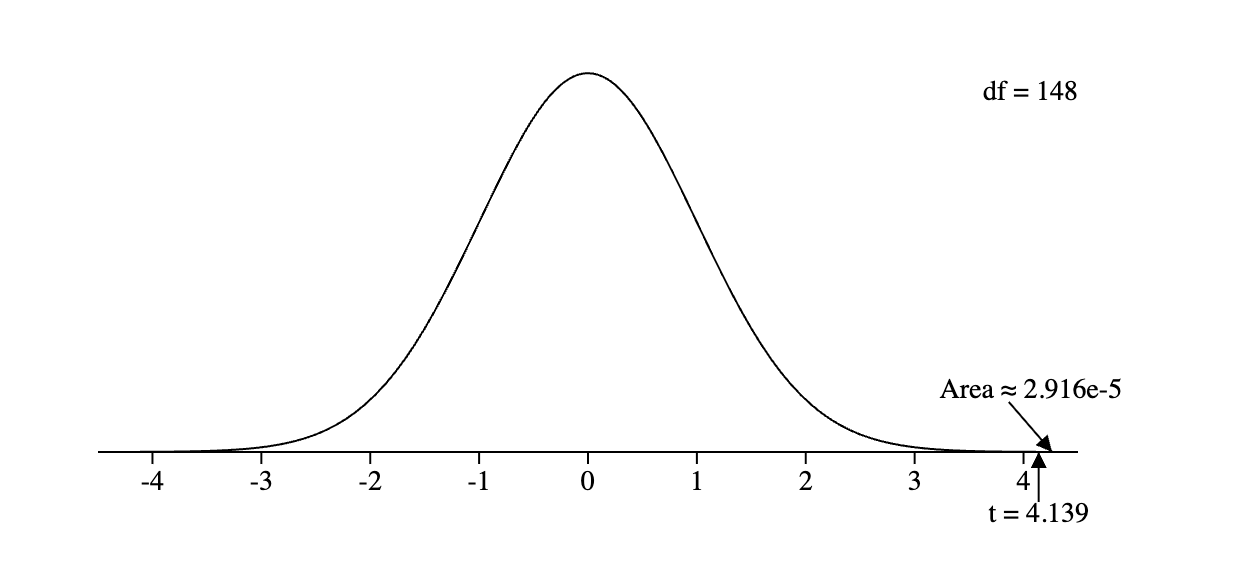
\includegraphics[width=0.7\textwidth]{Images/tdistribution}
        \caption{p-value calculation on a t-distribution with df = 148}
        \label{fig:t_dist}
    \end{figure}

    \noindent Based on the area under the curve in \textit{\autoref{fig:t_dist}} above $t=4.139$, our $p$-value is $2.916\cdot10^{-5}$.

    \section*{6. Conclusion}

    The $p$-value of $2.916\cdot10^{-5}$ indicates that, assuming that the population slope $\beta=0$, there is around a
    $0.002916\%$ probability of getting a sample slope as great or greater than our sample slope of $0.008312$, in a sample of
    150 randomly selected models from the population of convolutional models of our structure and of size 1 million parameters to 25 million parameters, trained
    on a randomly selected subset of 100 images from the CIFAR-10 train dataset and tested on the full test dataset of CIFAR-10.
    Because the $p$-value of $2.916\cdot10^{-5}$ is less than $\alpha=0.05$, we reject the null hypothesis, which states that the population slope $\beta$
    of the least-squares regression line that relates parameter count to difference in train and test accuracy (train - test) is $0$,
    in the population defined above.
    The data do provide convincing evidence that the population slope $\beta$ is greater than $0$, and that there is a positive correlation between
    parameter count and difference between train and test accuracy (train - test) in the population defined above.


    \section*{7. Reflection}

\end{document}
